\section{Data collection methodology}
\label{section:experiments}

We begin this section with a description of the enterprise network,
with the details of data capturing process to follow. According to 
Cisco documentation~\cite{cisco:ccent}, our network was two-tier 
medium-sized enterprise network comprising slightly more than 
$200$ workstations, one distribution switch (Cisco Catalyst 
G3560 series layer 3 switch), one router (the router was 
running Linux operating system) playing the role of a 
{\em VLAN router}, $6$ access switches from various vendors (1 DLink DES3200, 
1 Cisco 2690, 2 DLink DES1226 and 2 XNET SH9024 switches)
and also multiple, non-managed switches and one wireless 
access point all being connected to access switches.

%\begin{figure}[h!]
%\centering
%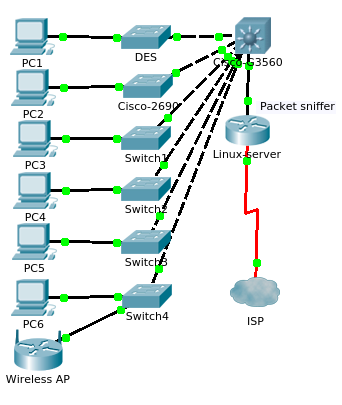
\includegraphics[width=0.4\textwidth]{graphics/network_arch.png}
%\caption{Enterprise network architecture}
%\label{fig:network}
%\end{figure}

Since we were unable to analyze fully the wiring of the access (especially those that were spread around the building and connected 
directly to access switches) and distribution switches, we could basically only guess (based on the limited information we had at our 
disposal) that there were no redundant links between access and distribution switches, also there were no redundant links between 
distribution switch and VLAN router. Essentially, the switches were merely connected in a tree like topology: each access switch was connected 
to one distribution switch, and the distribution switch was connected to a single router over a gigabit Ethernet trunk link. 

The entire network was partitioned into $25$ broadcast domains (VLANs), with native VLAN (VLAN that does not have tagging) being reserved 
for infrastructure management, although not all the switches were using native VLAN for management purposes. For bravity we omit discussion
about addressing in full detail, but rather mention that all VLANs were assinged addresses from class C private network from 
192.168.0.0 to 192.168.24.0, where as the last usable address in each subnetwork was used as the address for the default gateway. 
All hosts in the network used static address assignment schema.

To capture the traffic it was natural to put the sniffer at 
the central router, rather than installing it on multiple 
switches. With this respect, we configured sniffer at the 
router to capture the frames on a gigabit trunk interface.
We have used {\em tcpdump} to capture all traffic on the trunk 
link of a router - the link which was connected to 
the distribution switch. The data collection period 
lasted for slightly more than $2.5$ hours, from 
$06:23$ UTC to $09:03$ UTC and $19.1 \cdot 10^6$ 
frames were collected in total. Once the data was 
collected, a single {\em pcap} file was created. 
We then started to preprocess the captured data.
